\documentclass[]{report}
\usepackage{amssymb}
\usepackage{amsmath}
\usepackage{cancel}
\usepackage{xcolor}
\usepackage{tikz}
\usepackage{graphicx}
\usepackage{gensymb}
\newcommand\Ccancel[2][black]{\renewcommand\CancelColor{\color{#1}}\cancel{#2}}
\graphicspath{{./images/}}

\title{Precalculus Solutions}
\author{Michael Rocke}

\begin{document}

\maketitle

\tableofcontents

\section{Geometry}
\subsection{1}


\subsubsection{1}
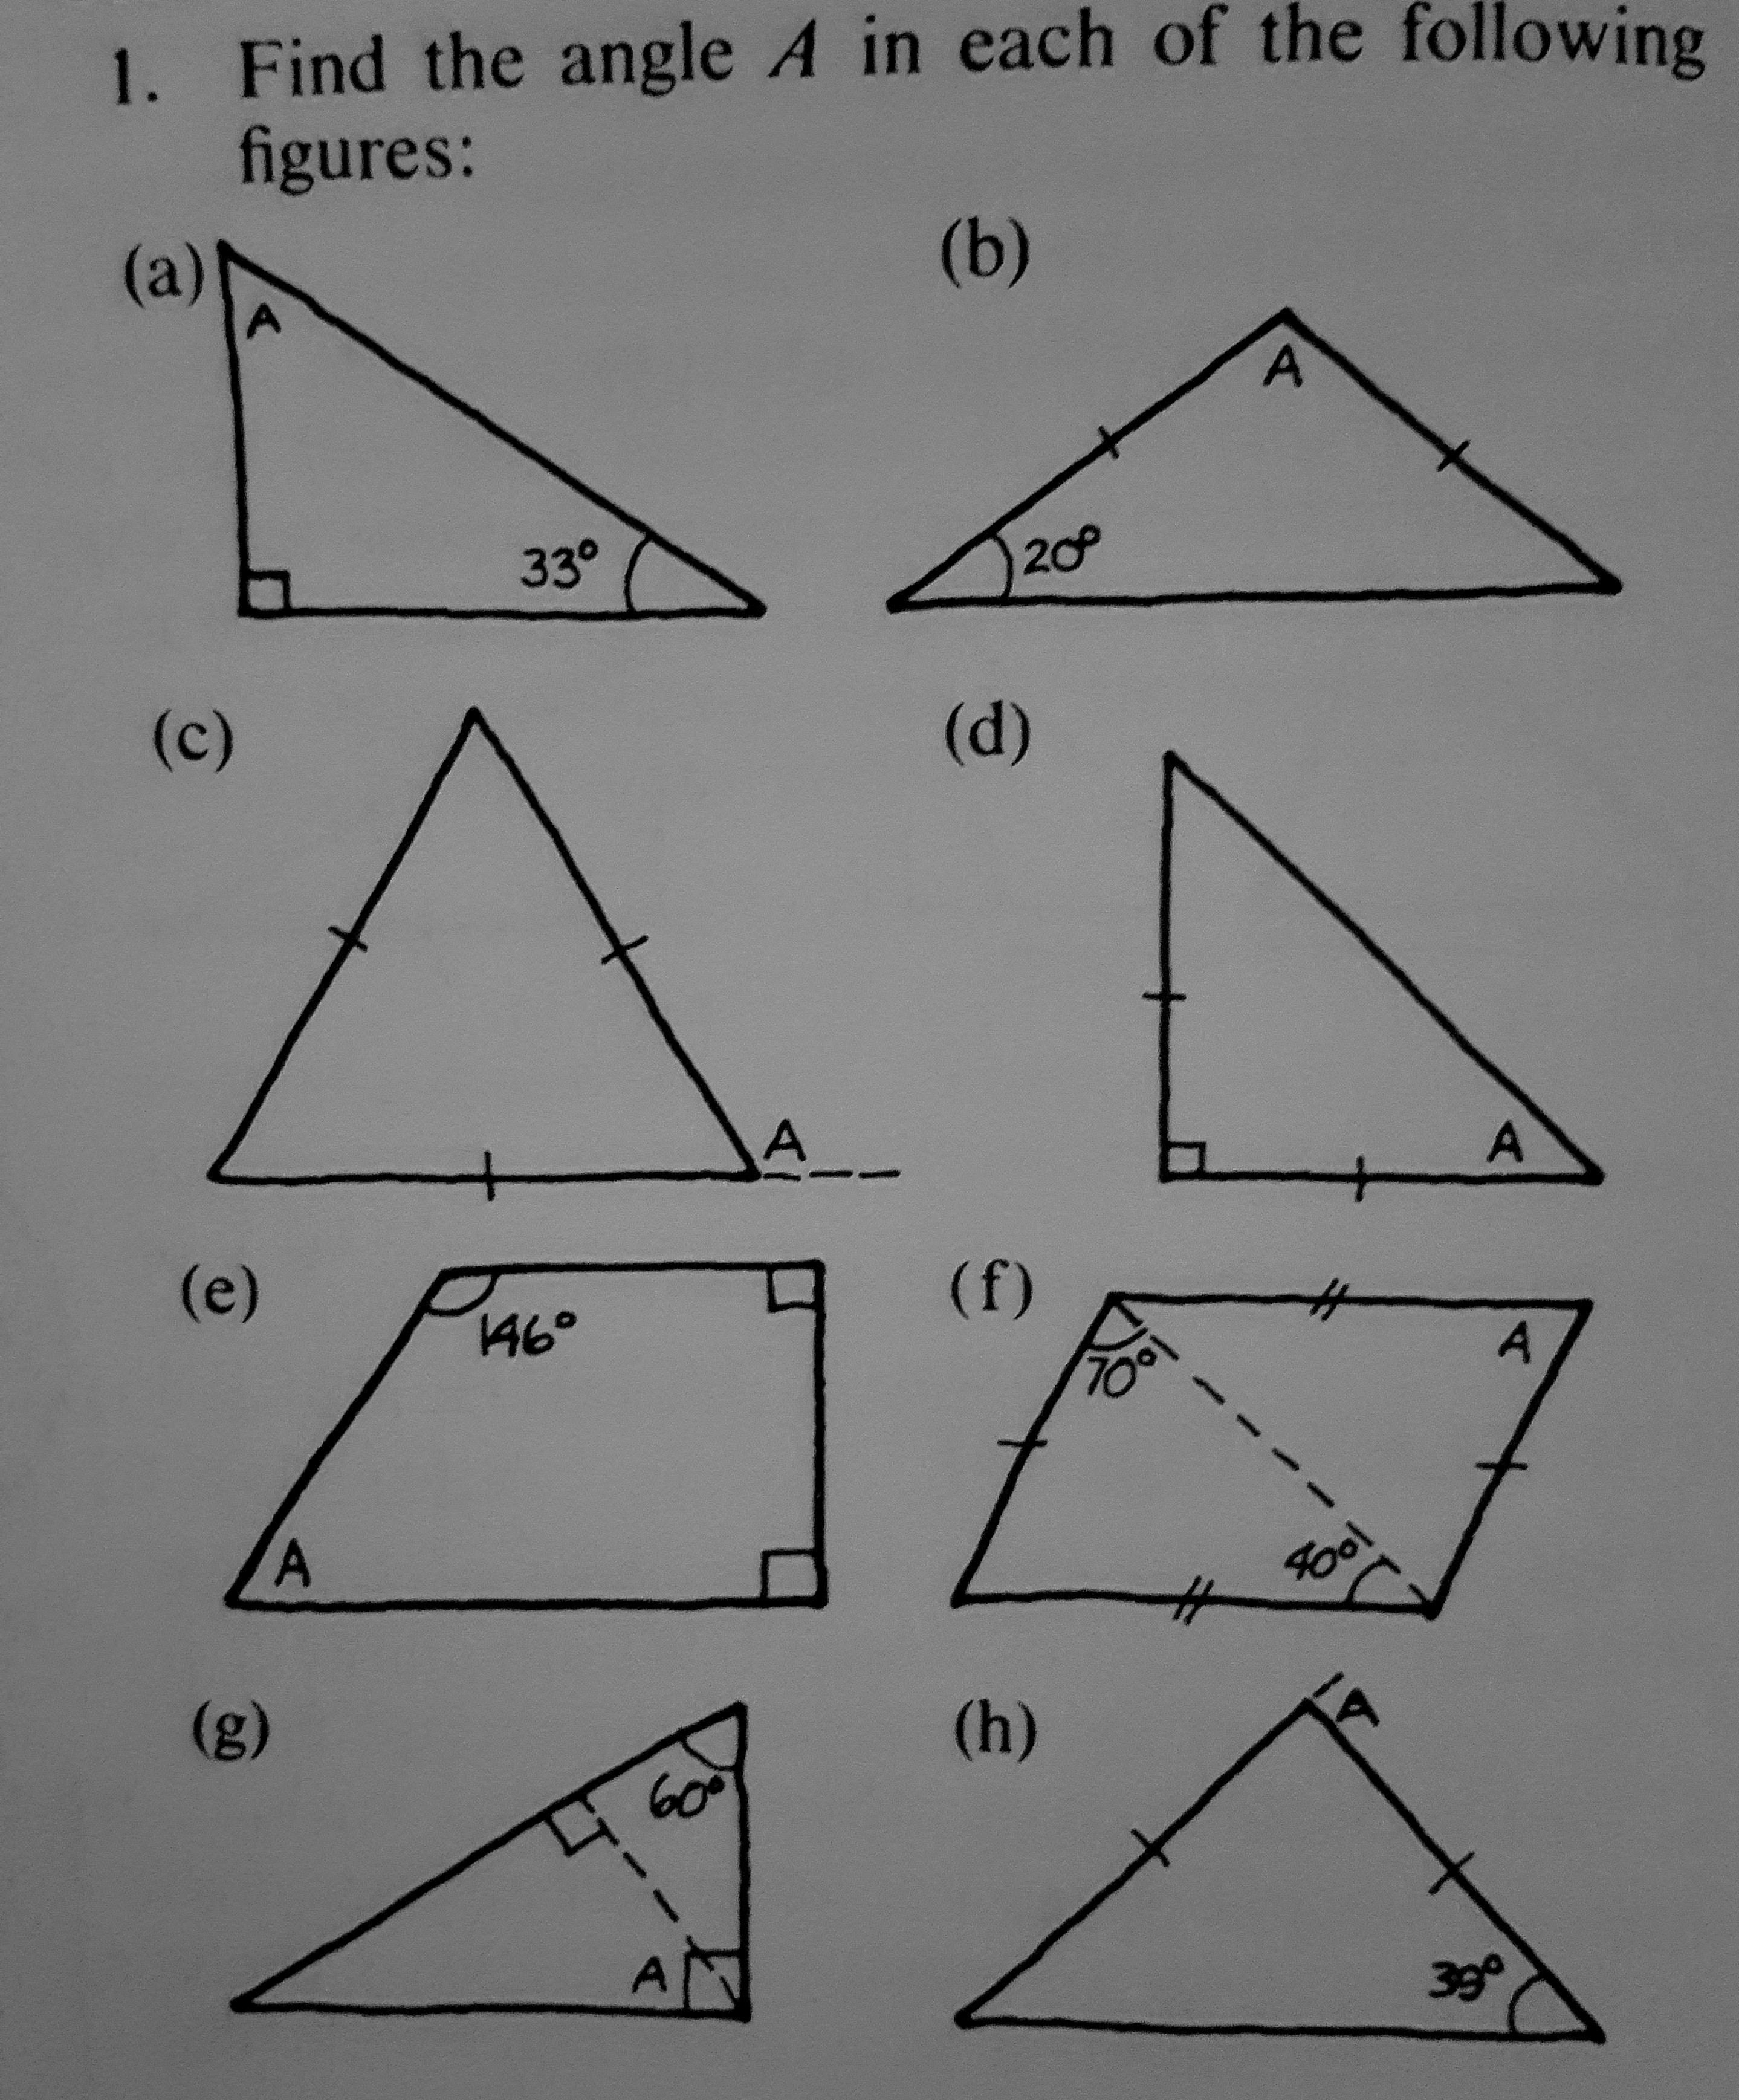
\includegraphics[width=\textwidth]{precalc-geo-section1-1.jpg}

a) $A = 180 - (90 + 33) = 57\degree$

b) $A = 180 - 2(20) = 140\degree$

c) $A = 180 - \frac{180}{3} = 120\degree$

d) $A = \frac{180 - 90}{2} = 45\degree$

e) $A = 180 - 90 - (146 - 90) = 90 -  56 = 34\degree$

f) $A = 180 - 70 - 40 = 70\degree$

g) $A = 90 - (180 - 60 - 90) = 60\degree$

h) $A = 180 - (180 - 2(39)) = 180 - 102 = 78\degree$
\subsubsection{2}

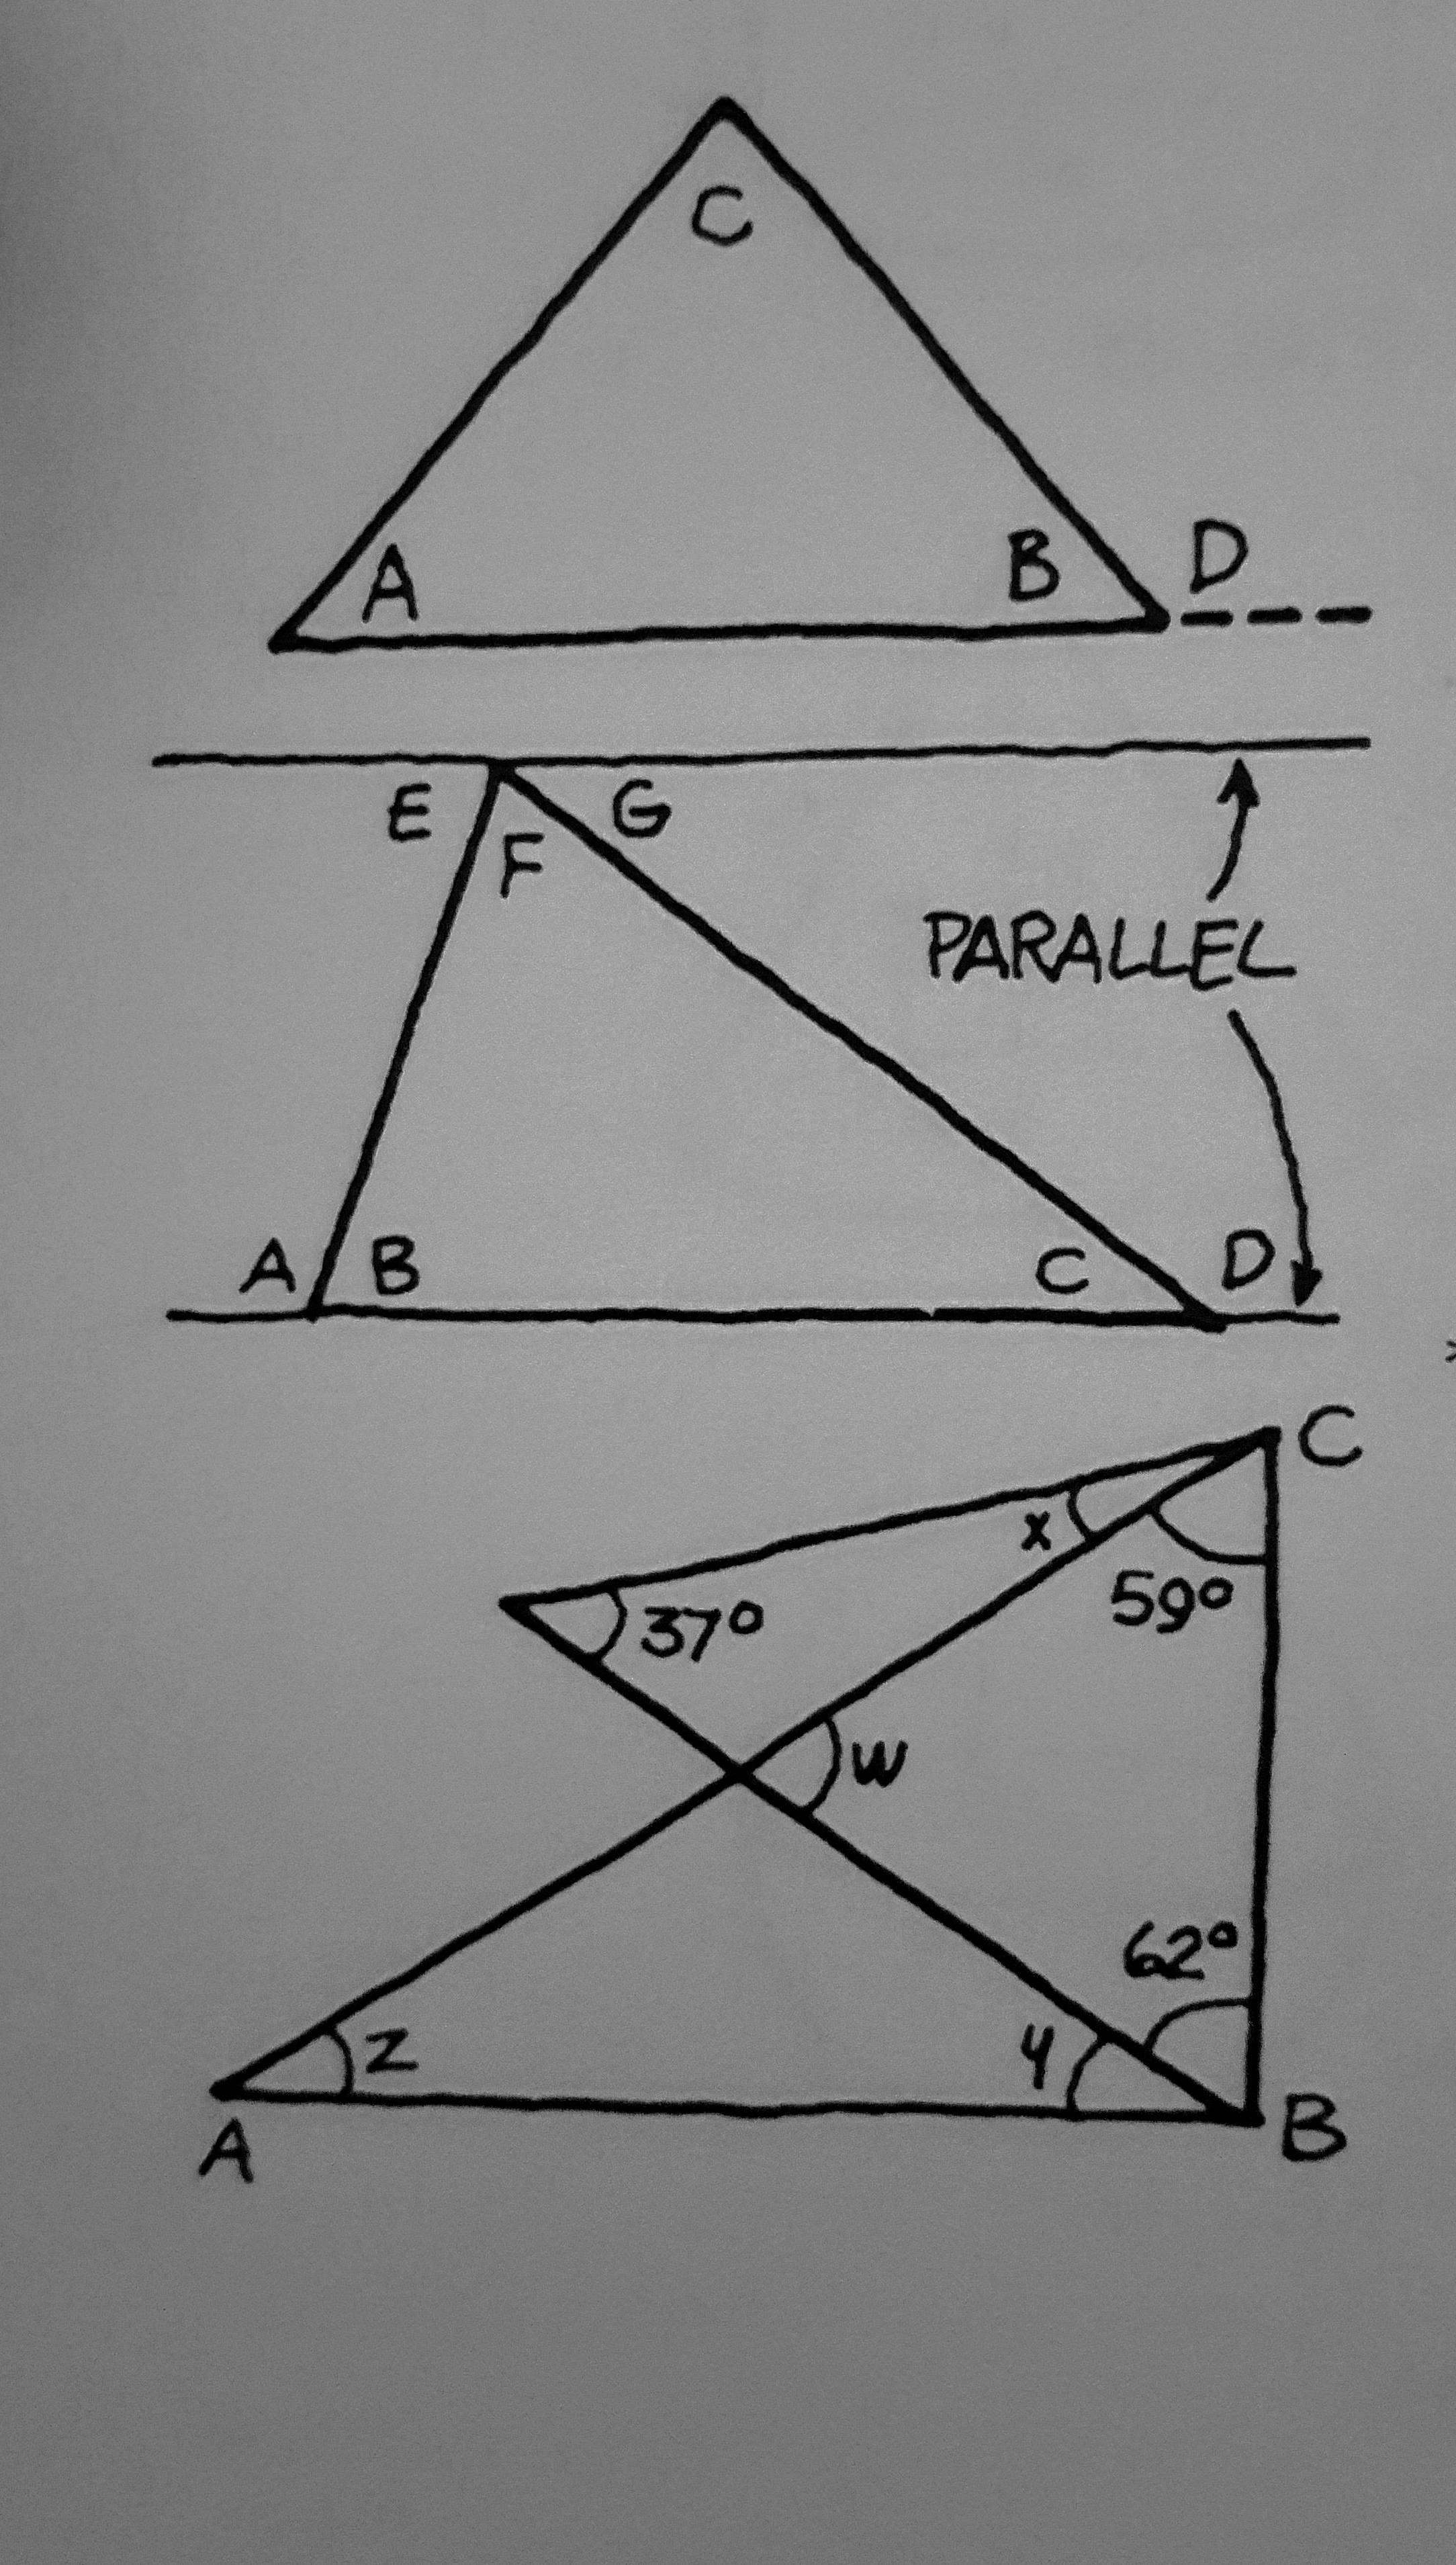
\includegraphics[width=\textwidth]{precalc-geo-section1-2.jpg}
In each case, for the first diagram, find the required angle;

a) $A=40\degree, C=100\degree, D=?$

\[
B = 180 - 40 - 100 = 40\degree; D = 180 - 40 = 140\degree;
\]

b) $A=50\degree, B=30\degree, C=?$

\[
C = 180 - 50 - 30 = 100\degree, D = 180 - 30 - 150\degree
\]

c) $A=50\degree, D=140\degree, C=?$
\[
B = 180 - 140 = 40\degree, C = 180 - 50 - 40 = 90\degree
\]


\subsubsection{3}

In each case, for the second diagram, find the angles not given;

a) $A=150\degree, C=40\degree$

\[
B = 180 - 150 = 30\degree, D = 180 - 40 = 140\degree, F = 180 - 30 - 40 = 110\degree, E=180-40-110=30\degree, G=40\degree
\]

b) $B=60\degree, C=65\degree$

\[
A = 180 - 60 = 120\degree, D=180-65=115\degree, E=60\degree, F=180-65-60 = 55\degree, G=65\degree
\]

\subsubsection{4}

In the third diagram, $AB \perp BC$ Find the angles $x, y, z, w$

\[
y=90-62=28\degree, w=180-59-62=59\degree, x=180-37-(180-59)=180-37-121=22\degree, z=180-59-(62+28)=31\degree 
\]

\subsubsection{5}
What is the height of a rectangle whose area is 40 square inches and whos base is 8 inches?

$area = 40 = 8h$

$h = \frac{40}{8}=5$

\subsubsection{6} 
If the base of a triangle is 9 inches, and its area is 45 square inches, what is the height?

\[
AreaOfTriangle=\frac{1}{2}\cdot base \cdot height
\]

\[
45 = \frac{1}{2} \cdot 9 \cdot h;
h = \frac{45\cdot2}{9} = \frac{90}{9} = 10
\]

\subsubsection{7}
The height and base of a triangle are equal, and its area is 32 square inches. Find the height and base.

\[
32 = \frac{1}{2}\cdot base^2;
base = \sqrt{64} = 8; height =8
\]

\section{Algebra}

\subsection{1}

\subsubsection{1}
$\sqrt{9} = 3^2$ - Integer or Natural Number\\
$-\frac{2}{3}$ - Rational \\
$ \frac{51}{3} = 17 $ - Integer or Natural Number \\
$ -10 $ - Integer \\
$ -\frac{\pi}{3} $ - Irrational \\
$ \frac{\sqrt{5}}{2} $ - Irrational \\
$ - \sqrt{4} = -2 $ - Integer \\
$ \frac{5}{1234} $ - Rational 

\subsubsection{2}
$ (3a - b)  - [2a - (a + b)] = (3a - b) - [2a - a - b] = (3a - b) - 2a + a + b = 3a - 2a + a - b + b = 2a $ \\


$ [(a + 3b) -a] - [a - (a - 3b)] =  [3b] -  [3b] = 0 $ \\



$ a - \{2a - [b - (3a - 2b)]\} = a  - \{2a - [3b - 3a]\} = a  - \{5a - 3b\} = a - 5a + 3b = 3b - 4a $

\subsubsection{3}
$ 19 \cdot 179 = 2(10 \cdot 179) - 179 = 2(1790) - 179 = 3580 - 179 = 3401 $ \\
$ 510 \cdot 18 = 2(10 \cdot 510) - (2 \cdot 510) = 10200 - 1020 = 9180 $ \\
$ 302 \cdot 11 = 10\cdot 302 + 302 = 3020 + 302 = 3322 $ \\

\subsubsection{4}

$ 12x - 18y + 30 = 6(2x - 3y + 5)$ \\
$ 8x^2 - 12x^3y - 28x^4z = 4x^2(2 - 3xy -7x^2z)$ \\
$ 9abc + 3a^2b^2c^2 = 3abc(3 + abc) $

\subsubsection{5}

$ \frac{a}{b} - \frac{b}{a} = \frac{a^2}{ab} - \frac{b^2}{ab} = \frac{a^2-b^2}{ab} $\\
$\frac{3}{x - 2}  + \frac{1}{2-x} = \frac{3(2-x) + (x-2)}{(x-2)(2-x)} = \frac{4 - 2x}{(x-2)(2-x)} =\frac{2\cancel{(2 - x)}}{(x-2)\cancel{(2-x)}} = \frac{2}{x-2}$\\


$\frac{1}{1 + \frac{1}{x-1}} = \frac{1}{\frac{x-1}{x-1} + \frac{1}{x-1}} = \frac{1}{\frac{x\cancel{-1+1}}{x-1}} = \frac{x-1}{x}$ \\

using an example of x = 2;
$\frac{1}{2} $ 

using an example of x = 3;
$\frac{2}{3} $ 



$\frac{x}{xy^2} + \frac{y}{x^2y} = \frac{x^3y + xy^3}{x^3y^3} = \frac{x^2 + y^2}{x^2y^2}$ \\
$\frac{4a}{b} + \frac{b}{4a} = \frac{16a^2 + b^2}{4ab}$

\subsubsection{6}

a) $5a^{-3}  =  \frac{5}{a^3}$ \\
b) $(5a)^{-3} = \frac{1}{125a^3}$ \\
c) $21 \cdot 719^3 \cdot 7^{-1} \cdot 3 \cdot 719^{-3} = 21 \cdot \cancel{719^3} \cdot \frac{1}{7} \cdot 3 \cdot \cancel{719^{-3}}  = \frac{27 \cdot 3}{7} = 3^2$ \\
d) 1 \\

\subsubsection{7}
a)  $(a^{n-4}b^4)(ab^{n-1})^4 = (a^{n-4}b^4)(a^4b^{4n -4}) = a^nb^{4n}$ \\
b)  $(4a^3b^{-4})(3a^{-1}b^5) = 12a^2b$ \\
c)  $\frac{x^{14}y^5}{x^4y^{-5}} = x^{10}y^{10}$ \\z
d)  $a^2b^2(a^{-2} + b^{-2}) = b^2 + a^2$ \\
e)  $(x+y)(x^{-1} + y^{-1}) =  (x+y)(\frac{1}{x}+\frac{1}{y}) = (x+y)(\frac{y + x}{xy}) = (\frac{x^2 + 2yx + y^2}{xy})$ \\

Using x = 2, y = 3;
$5 (\frac{1}{2}+\frac{1}{3}) = 5 (\frac{5}{6}) = \frac{25}{6}$

f)  $(\frac{a^2b}{c})^4(\frac{a}{b^2c^3})^2(\frac{c^2}{a^2})^5 = (\frac{a^8b^4}{c^4})(\frac{a^2}{b^4c^6})(\frac{c^{10}}{a^{10}}) = \frac{a^{10}b^4c^{10}}{c^{10}b^4a^{10}} = 1$ \\


\subsubsection{8}
Simplify


a) $\sqrt{49} = 7$


b) $\sqrt{144} = 12$

c) $\sqrt{9  + 16} = \sqrt{25} = 5$

d) $\sqrt{36+ 64} = \sqrt{100} = 10$

e) $\sqrt[3]{27} = 3$

f) $\sqrt[4]{81} = 3$

g) $\sqrt[6]{64} = 2$

h) $\sqrt{.64} = \sqrt{\frac{64}{100}} = \frac{8}{10} = 0.8$

i) $\sqrt{.09} = \frac{3}{10} = .3$

j) $\sqrt{\frac{16}{121}} = \frac{\sqrt{16}}{\sqrt{121}} = \frac{4}{11}$

k) $\sqrt{\frac{225}{400}} = \frac{15}{20} = \frac{3}{4}$

l) $\sqrt[3]{-\frac{1}{27}} = -\frac{1}{3}$

m) $\sqrt[3]{\frac{64}{125}} = \frac{4}{5}$

n) $\sqrt[3]{-1000} = -10$ 

o) $\sqrt{125} = \sqrt{5 * 5 * 5} = 5\sqrt{5}$

p) $\sqrt{625} = 25$

q) $\sqrt[4]{625} = \sqrt[4]{25 * 25} = \sqrt[4]{5 * 5 * 5 * 5} = 5$

r) $\sqrt{18} = \sqrt{2 * 9} = 3\sqrt{2}$

s) $\sqrt{12} = \sqrt{4 * 3} = 2\sqrt{3}$

t) $\sqrt{2} + \sqrt{8} = \sqrt{2} + 2\sqrt{2} = 3\sqrt{2}$

u) $\sqrt{3} + \sqrt[4]{9} =  \sqrt{3} + \sqrt[4]{\sqrt{3} * \sqrt{3} * \sqrt{3} * \sqrt{3}} = 2\sqrt{3} $

v) $\sqrt[3]{54} + \sqrt[3]{250} = \sqrt[3]{3 * 3 * 3 * 2 } + \sqrt[3]{5 * 5 * 5 *2} = 3\sqrt[3]{2} + 5\sqrt[3]{2}  = 8\sqrt[3]2$

w) $\sqrt[10]{32a^5} = \sqrt[10]{2^5a^5} = \sqrt{2a}$

x) $\sqrt{a^2b^4} = ab^2$

y) $\sqrt[4]{a^5} = \sqrt[4]{a * a * a * a * a} = a \sqrt[4]{a}$

z) $\sqrt{1 - (\frac{\sqrt{3}}{2})^2} = \sqrt{1 - (\frac{3}{4})} = \sqrt{\frac{1}{4}}  = \frac{1}{2}$

\subsubsection{9}
Simplify by rationalizing the denominator


a) $\frac{30}{\sqrt{6}} = \frac{30}{\sqrt{6}} \cdot \frac{\sqrt{6}}{\sqrt{6}} = \frac{30\sqrt{6}}{6} = 5\sqrt{6}$

b) $\frac{\sqrt{6} + 2}{\sqrt{6} - 2} = \frac{\sqrt{6} + 2}{\sqrt{6} - 2} \cdot \frac{\sqrt{6} + 2}{\sqrt{6} + 2} = \frac{6 + 4\sqrt{6} + 4}{6 - 4} = \frac{10 + 4\sqrt{6}}{2} = 5 + 2\sqrt{6}$


c) $\frac{2}{\sqrt{7} + \sqrt{5}} = \frac{2}{\sqrt{7} + \sqrt{5}} \cdot  \frac{\sqrt{7} - \sqrt{5}}{\sqrt{7} - \sqrt{5}} = \sqrt{7} - \sqrt{5}$
	
\subsubsection{10}
Compute

a) $36^{\frac{1}{2}} = 6$

b) $8^{\frac{1}{3}} = 2$

c) $32^{\frac{4}{5}} = \sqrt[5]{32^4} = 16$

d) $36^{\frac{3}{2}} = 216$	

e) $216^{\frac{2}{3}} = 36$

f) $16^{-\frac{1}{2}} = (\frac{1}{16})^{\frac{1}{2}} = (\frac{1}{\sqrt{16}}) = \frac{1}{4}$

g) $ 9^{-3/2} = \frac{1}{9}^{3/2} = \frac{1}{27}$

h) $8^{-2/3} = \frac{1}{8}^{2/3} = \frac{1}{4}$

i) $ 100^{3/2} = \sqrt[2]{100^3} = 1000$

j) $3^{1/2} \cdot 3^{5/2} = 3^{\frac{1}{2} + \frac{5}{2}} = 3^{\frac{6}{2}} = 3^3 = 27$

k) $\frac{10^{2/3} \cdot 10^{1/3} \cdot 10^3}{10^{5/2} \cdot 10^{1/2}} = \frac{10^4}{10^3} = 10$

\subsubsection{11}
Simplify as far as possible, removing negative and zero exponents

a) $(25a^6b^{-2})^{1/2} = \frac{5a^3}{b}$


b) $(2a^{1/2}b^{1/4})^4 = 16a^2b$

c) $\sqrt[5]{a^2b} \cdot \sqrt[5]{a^3b^4} = (a^2b \cdot a^3b^4)^{1/5} = (a^5b^5)^{1/5} = ab$

d) $(\frac{a^4}{36})^{1/2} = \frac{a^2}{6}$

e) $(25a^{2/3})^{1/2} = 5a^{1/3} = 5\sqrt[3]{a}$

f) $(a^{1/2} + b^{1/2})(a^{1/2} - b^{1/2}) = a - b$

g) $\{a^{2/3} [(\frac{a^{2/3}}{a^{1/4}})^6]^{1/3}\}^2 = \{a^{4/3} [(\frac{a^{2/3}}{a^{1/4}})^6]^{2/3}\} = \{a^{4/3} [(\frac{a^{2/3}}{a^{1/4}})^4]\} = \{a^{4/3} [(\frac{a^{8/3}}{a})]\} =  \{a^{4/3} a^{5/3}\} = a^{9/3} = a^3$

h) $(\frac{27b^2c^5}{64a^6b^{-4}c^{-1}})^{1/3} =  \frac{3b^{2/3}c^{5/3}}{4a^2b^{-4/3}c^{-1/3}} = \frac{3b^2c^2}{4a^2}$



\subsubsection{12}

Add or subtract


a) $(x^7 - 3x^5 + 4x^2 - 9) + (2x^6 - 5x^5 - 2x^4 + x^3 - 2x^2 + x + 1) = x^7 + 2x^6 - 8x^5 - 2x^4 + x^3 + 2x^2 - 8$

b) $(3x^5 + x^4 - 2x^3 + 5x^2 - 11x + 2) - (x^4 + 5x^2 + 2) = 3x^5 - 2x^3 - 11x$


\subsubsection{13}
Multiply

a) $(2x^3 + 3x^2 - 4)(3x^2 - 2x - 9) = 6x^5 - 4x^4 - 18x^3 + 9x^4 - 6x^3 - 27x^2 - 12x^2 + 8x + 36 = 6x^5 + 5x^4 - 24x^3 - 39x^2 + 8x + 36$

b) $(x^5 - 2x^3 + 3)(2x^2 - 8x + 4) = 2x^7 - 8x^6 + 4x^5 - 4x^5 + 16x^4 - 8x^3 + 6x^2 - 24x + 12 =  2x^7 - 8x^6 + 16x^4 - 8x^3 + 6x^2 - 24x + 12$

c) $(x-1)(x^2 + x + 1) = x^3 + x^2 + x - x^2 - x - 1 = x^3 - 1$

d) $(x-1)(x^3 + x^2 + x + 1) = x^4 + x^3 + x^2 + x - x^3 - x^2 - x - 1 = x^4 -1$

e) $(x-1)(x^4+x^3+x^2+x+1) = x^5 - 1$

\subsubsection{14}

Factor 

a) $x^2 -x - 6 = (x+2)(x-3)$

b) $x^2 + 9x + 20 = (x + 5)(x + 4)$

c) $x^2 + 12x + 20 = (x + 10)(x + 2)$

d) $x^2 -4x + 4 = (x-2)(x-2) = (x-2)^2$

e) $x^2 + 8x + 16 = (x+4)^2$

f) $x^3 + 12x^2 + 36x = x(x^2 + 12x + 36) = x(x+6)^2$

g)$x^4 - 16 = (x^2+4)(x-2)(x+2)$

h) $x^2 + 13x - 30 = (x+15)(x-2)$

i) $x^2 + 2x - 35 =  (x-5)(x+7)$

j) $x^2 - 13x + 42 = (x - 6)(x - 7)$

k) $x^3 - 3x^2 - 4x = x(x^2 - 3x - 4) = x(x-4)(x + 1)$

l) $4x^2 + 2x - 12 = (2x - 3)(2x+4) $

m) $10x^2 - 16x - 8 = (10x + 4)(x - 2)$

\subsubsection{15}

Verify the formula $(x-a)(x^2 + ax + a^2) = x^3 - a^3$

$(x-a)(x^2 + ax + a^2) = x^3 \Ccancel[red]{+ ax^2 } \Ccancel[blue]{+ a^2x}  \Ccancel[red]{- ax^2}  \Ccancel[blue]{- a^2x} - a^3 = x^3 - a^3$

a) $x^3 - 27 = (x^3 - 3^3) =(x-3)(x^2 + 3x + 3^2)  $

b) $8x^3 - 125 = (2x-5)(4x^2 + 10x + 25) $


\subsubsection{16}


Verify the formula $(x+a)(x^2 - ax + a^2) = x^3 + a^3$
$(x+a)(x^2 - ax + a^2) = x^3  \Ccancel[red]{- ax^2} \Ccancel[blue]{+ a^2x} \Ccancel[red]{+ ax^2} \Ccancel[blue]{- a^2x} + a^3$


and use to factor

a) $x^3 + 64 = x^3 + 4^3 = (x+4)(x^2 - 4x + 16)$

b) $27x^3 + 8 = (3x)^3 + 2^3 = (3x + 2)(9x^2 - 6x + 4)$

\subsubsection{17}

Solve by factoring, and then by quadratic forumla

Quadratic formula;

$x = \frac{-b \pm \sqrt{b^2 - 4ac}}{2a}$

a) $x^2 + 3x - 28 = 0 = (x + 7)(x - 4)$

or using Quadratic formula;
\[
let a = 1, b = 3, c = -28 \\
\]

\[
x = \frac{-3 \pm \sqrt{(-3)^2 - 4\cdot1\cdot-28}}{2\cdot1} = \frac{-3 \pm \sqrt{9 + 112}}{2} = \frac{-3 \pm 11}{2}
\]

\[
x = \frac{8}{2} = 4 ,  \frac{-14}{2} = -7
\]

b) $x^2 - 8x - 33 = 0 = (x + 3)(x - 11)$

or using Quadratic formula

\[
let a=1, b=-8, c= -33
\]

\[
x = \frac{-(-8) \pm \sqrt{(-8)^2 - 4\cdot1\cdot(-33)}}{2\cdot1} = \frac{8 \pm \sqrt{64  + 132}}{2} = \frac{8 \pm \sqrt{196}}{2} = \frac{8 \pm 14}{2}
\]

\[
x = \frac{-6}{2}, \frac{22}{2}
\]



c) $2x^2 + x -15 = 0 = (2x - 5)(x + 3)$


or  using Quadratic formula

\[
let a=2, b=1, c=-15
\]

\[
x = \frac{-1 \pm \sqrt{1^2 - 4\cdot2\cdot(-15)}}{2\cdot2} = \frac{-1 \pm \sqrt{1 + 120}}{4} = \frac{-1 \pm 11}{4}
\]

\[
x = \frac{-12}{4} = -3, \frac{10}{4}
\]

d) $6x^2 - 5x -21 = 0 = (3x - 7)(2x + 3)$

or using Quadratic Formula

\[
let a=6, b=-5, c=-21
\]

\[
x = \frac{-(-5) \pm \sqrt{(-5)^2 - 4\cdot6\cdot(-21)}}{2\cdot6} = \frac{5 \pm \sqrt{529}}{12} = \frac{5 \pm 23}{12}
\]

Thus

\[
x=\frac{-18}{12} = \frac{-3}{2}, \frac{28}{12} = \frac{7}{3}
\]



\subsubsection{18}

Solve by the quadratic formula

a) $5x^2 - 9x + 3 = 0 $

\[
x = \frac{-(-9) \pm \sqrt{(-9)^2 - 4\cdot5\cdot3}}{2\cdot5} = \frac{9 \pm \sqrt{21}}{10}
\]

b) $3x^2 + 7x + 3 = 0$

\[
x = \frac{-7 \pm \sqrt{7^2 - 4\cdot3\cdot3}}{2\cdot3} = \frac{-7 \pm \sqrt{13}}{6}
\]

c) $17x^2 - 6x + 1 = 0$

\[
x = \frac{-(-6) \pm \sqrt{(-6)^2 - 4\cdot17\cdot1}}{2\cdot17} = \frac{6 \pm \sqrt{-32}}{34}
\]

x has no real values, because you cannot sqaure root a negative number


d) $x^2 + x + 1 = 0$

\[
x = \frac{-1 \pm \sqrt{1 - 4\cdot1\cdot1}}{2} = \frac{-1 \pm \sqrt{-3}}{2}
\]

x has no real values, because you cannot sqaure root a negative number

\subsubsection{19}

Insert the correct inequality sign, < or > in the following;

a) $ 3 < 11$

b) $5 > 2$

c) $-4 < -3 $

d) $-6 < -2$

e) $-2 > -3$

f) $\pi < 2\sqrt{3}$

\subsubsection{20}

Solve the linear inequalities

a) $ 5-2x > 17 $

\begin{align*}
5-2x > 17  \\
-2x > 17 - 5 > 12 \tag*{taking 5 off}\\
-x > 6 \tag*{dividing by 2}\\
x < -6 \tag*{multiplying by -1}
\end{align*}

b) $ 3x + 4 > 13$

\begin{align*}
3x + 4 > 13 \\
3x > 9 \tag*{taking 4 off}\\
x > 3 \tag*{dividing by 3}
\end{align*}

\subsubsection{21}

Solve the equations

a) $|x| = 2 $

\[
x = \pm 2
\]

b) $|2x| = 6$

\[
x = \pm 3
\]
c) $|\frac{1}{3}x| = 2 $
\[
x = \pm 6
\]

d) $|x-2| = 3 $

\[
x = -1 or 5
\]

e) $|x + 3 | = 1$

\[
x = -4, -2
\]

\subsubsection{22}

Solve the quadratic inequality $x(x-1) > 0$ by noticing that both factors must be positive or both factors must be negative

\[
x < 0 , x > 1
\]

\subsubsection{23}
Solve the quadratic inequality $x^2 + 2x - 15 > 0$ by noticing that both factors must be positive or both factors must be negative

\[
x^2 + 2x - 15  = (x - 3)(x + 5)
x < -5, x > 3
\]

\subsection{2} Functions and Graphs

\subsubsection{1}
if $f(x) = 4x-3$, find $f(0), f(1), f(2), f(3)$

\begin{align*}
f(0) = 4\cdot0 - 3 = -3\\
f(1) = 4\cdot1 - 3 = 1 \\
f(2) = 4\cdot2 - 3 = 5 \\
f(3) = 4\cdot3 - 3 = 9
\end{align*}

\subsubsection{2}
if $g(x) = \frac{2x-4}{3x^2 + 1}$ find $g(0), g(1), g(-\frac{1}{2})$


\begin{align*}
g(0) = \frac{2\cdot0-4}{3\cdot0^2 + 1} = \frac{-4}{1} = -4\\
g(1) = \frac{2\cdot1 - 4}{3\cdot1^2 + 1} = \frac{-2}{4} = -\frac{1}{2}\\
g(-\frac{1}{2}) = \frac{2\cdot(-\frac{1}{2}) - 4}{3\cdot(-\frac{1}{2})^2 + 1} = \frac{-5}{\frac{7}{4}} = -\frac{20}{7}
\end{align*}


\subsubsection{3}
if $h(x) = x^3 - 3x^2 + 5x - 1$, find $h(x^3)$

\[
(x^3)^3 - 3(x^3)^2 + 5(x^3) - 1 = x^9 - 3x^6 + 5x^3 - 1
\]

\subsubsection{4}

if $F(x) = \frac{x}{x-1}$ find $F[F(x)]$


\[
F(\frac{x}{x-1}) = \frac{\frac{x}{x-1}}{\frac{x}{x-1}-1} = \frac{x}{x-1} \cdot \frac{1}{\frac{x}{x-1}-1} =  x
\]

\subsubsection{5}

Express the area A of a square as a function of 

a) the length of one side x

\[
Area(x) = x^2
\]

b) the perimeter p
\[
Area(p) = (\frac{p}{4})^2
\]

\subsubsection{6}

Express the area A of a circle as a function of its circumference c

\[
Circumference(d) = \pi \cdot d;
Radius(c) = \frac{c}{\pi \cdot 2};
Area(c) = \pi (\frac{c}{\pi \cdot 2})^2 = \pi \frac{c^2}{\pi^2 \cdot 4} = \frac{c^2}{4\pi}
\]

\subsubsection{7} TODO
Express the height of an equilateral triangle as a function of the base x

\[
Height(x) = \sqrt{x^2 - (\frac{x}{2})^2}
\]

\subsubsection{8}
Two cyclists start racing along a straight road from the same place at the same time in the same direction.

If one travels 40 mi/hr and the other 35 mi/hr, find the distance between them $t$ hours after they start

\[
Distance(t) = (40\cdot t) - (35\cdot t) = 5t
\]

\subsubsection{9}

Draw the triangle having the following points as vertices;

a) $(1, -1), (4, 2), (-3, 5)$

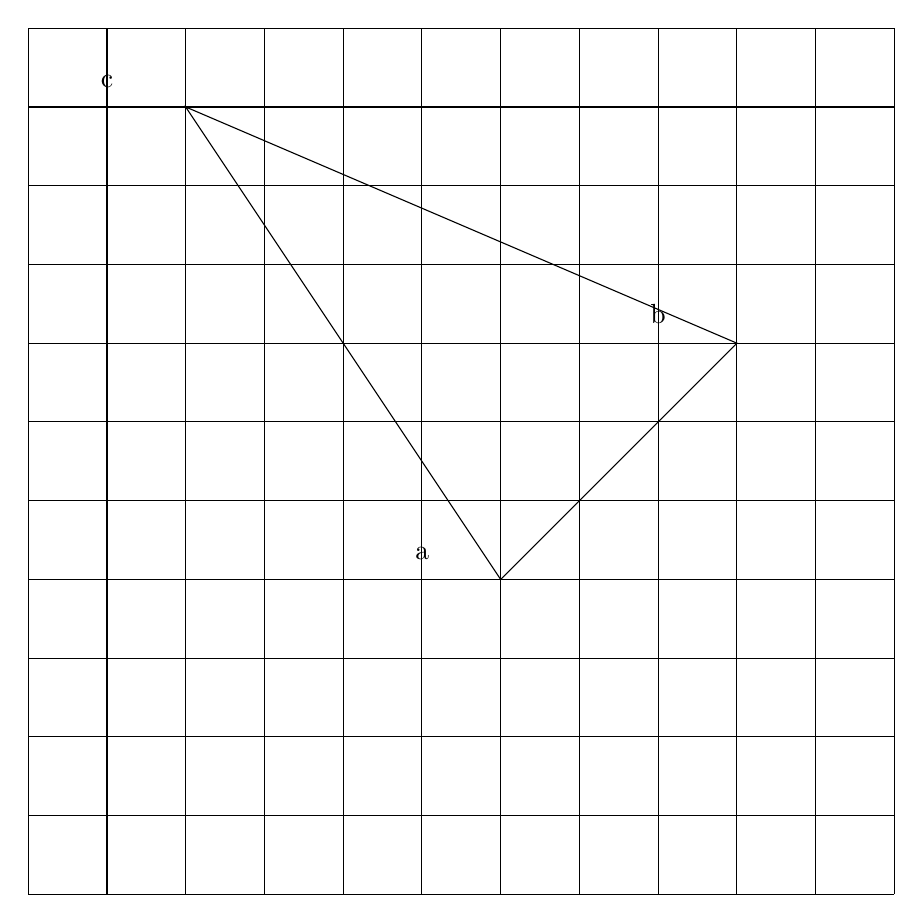
\begin{tikzpicture}
	\draw (-5, -5) grid (6, 6);
	
	\coordinate (a) at (1, -1);
	\coordinate (b) at (4, 2);
	\coordinate (c) at (-3, 5);
	
	\node[label=above:a, left of=a](a){};
	
	\node[label=above:b, left of=b](b){};
	\node[label=above:c, left of=c](c){};
	
	\draw (1, -1) -- (4, 2) -- (-3, 5) -- cycle;
\end{tikzpicture}

b) $(5, -2)(-2, -4), (1, 4)$

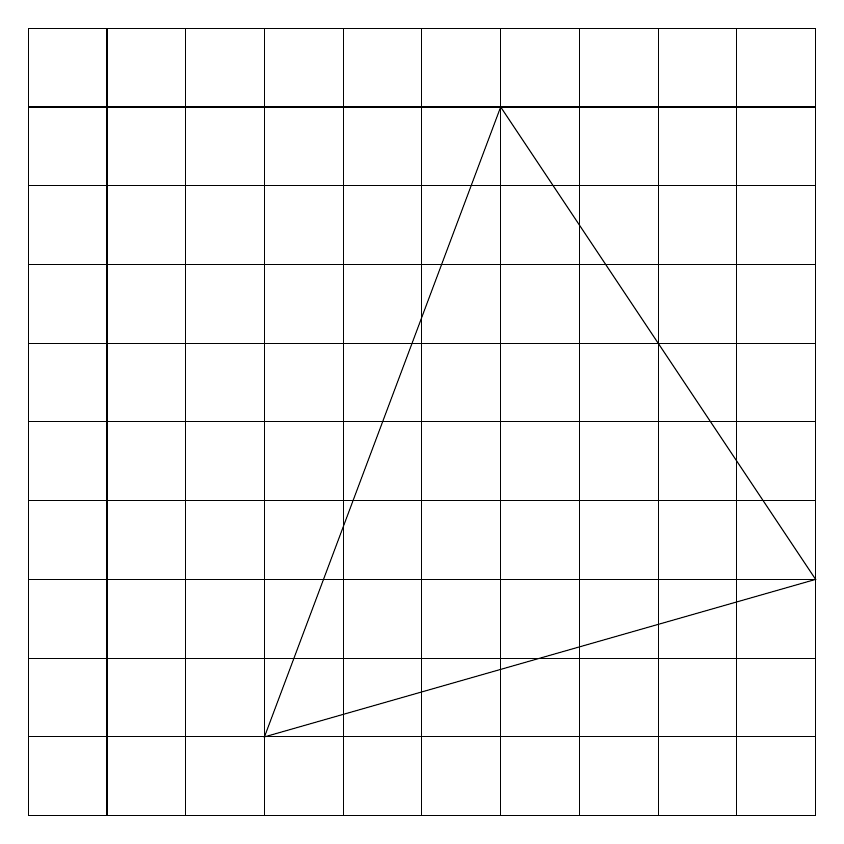
\begin{tikzpicture}
\draw (-5, -5) grid (5, 5);

\coordinate (a) at (5, -2);
\coordinate (b) at (-2, -4);
\coordinate (c) at (1, 4);

\draw (a) -- (b) -- (c) -- cycle;


\end{tikzpicture}


\subsubsection{10}

Find the length of the sides and the hypotenuse of the right triangle whos vertices are;

a) (1, 2), (-3, 2), (-3, 5)

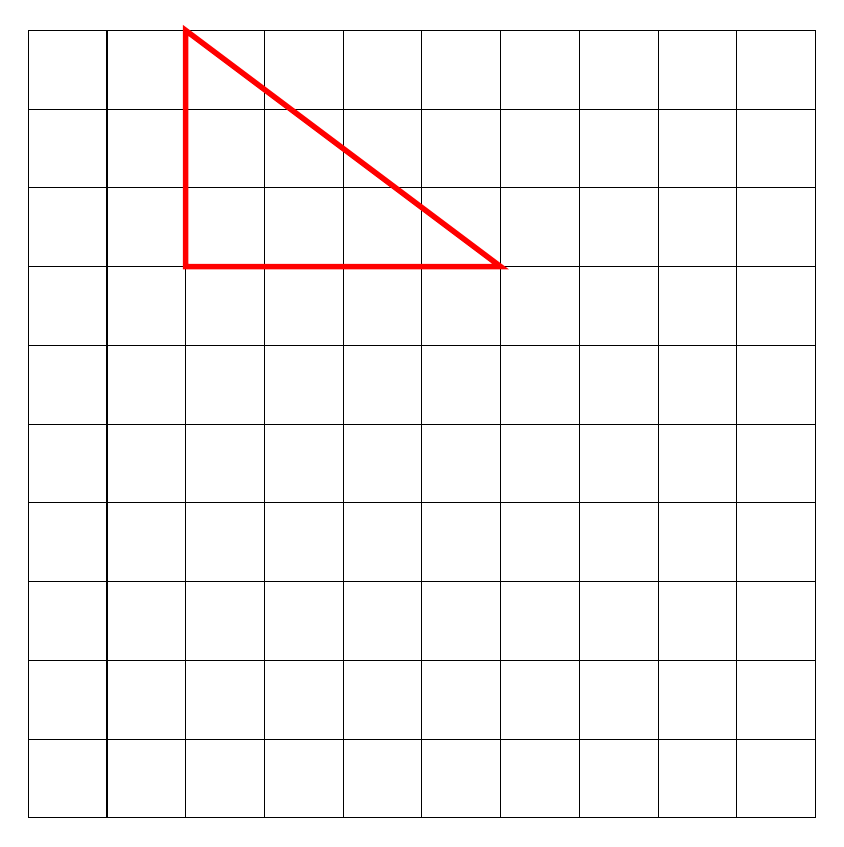
\begin{tikzpicture}
\draw (-5, -5) grid (5, 5);

\coordinate (a) at (1, 2);
\coordinate (b) at (-3, 2);
\coordinate (c) at (-3, 5);

\draw [line width=2pt, red] (a) -- (b) -- (c) -- cycle;

\end{tikzpicture}

\[
height = 3, base = 4, hypotenuse = \sqrt{3^2 + 4^2} = \sqrt{9 + 16} = \sqrt{25} = 5
\]

b) (2, -5), (2, 7), (-3, 7)

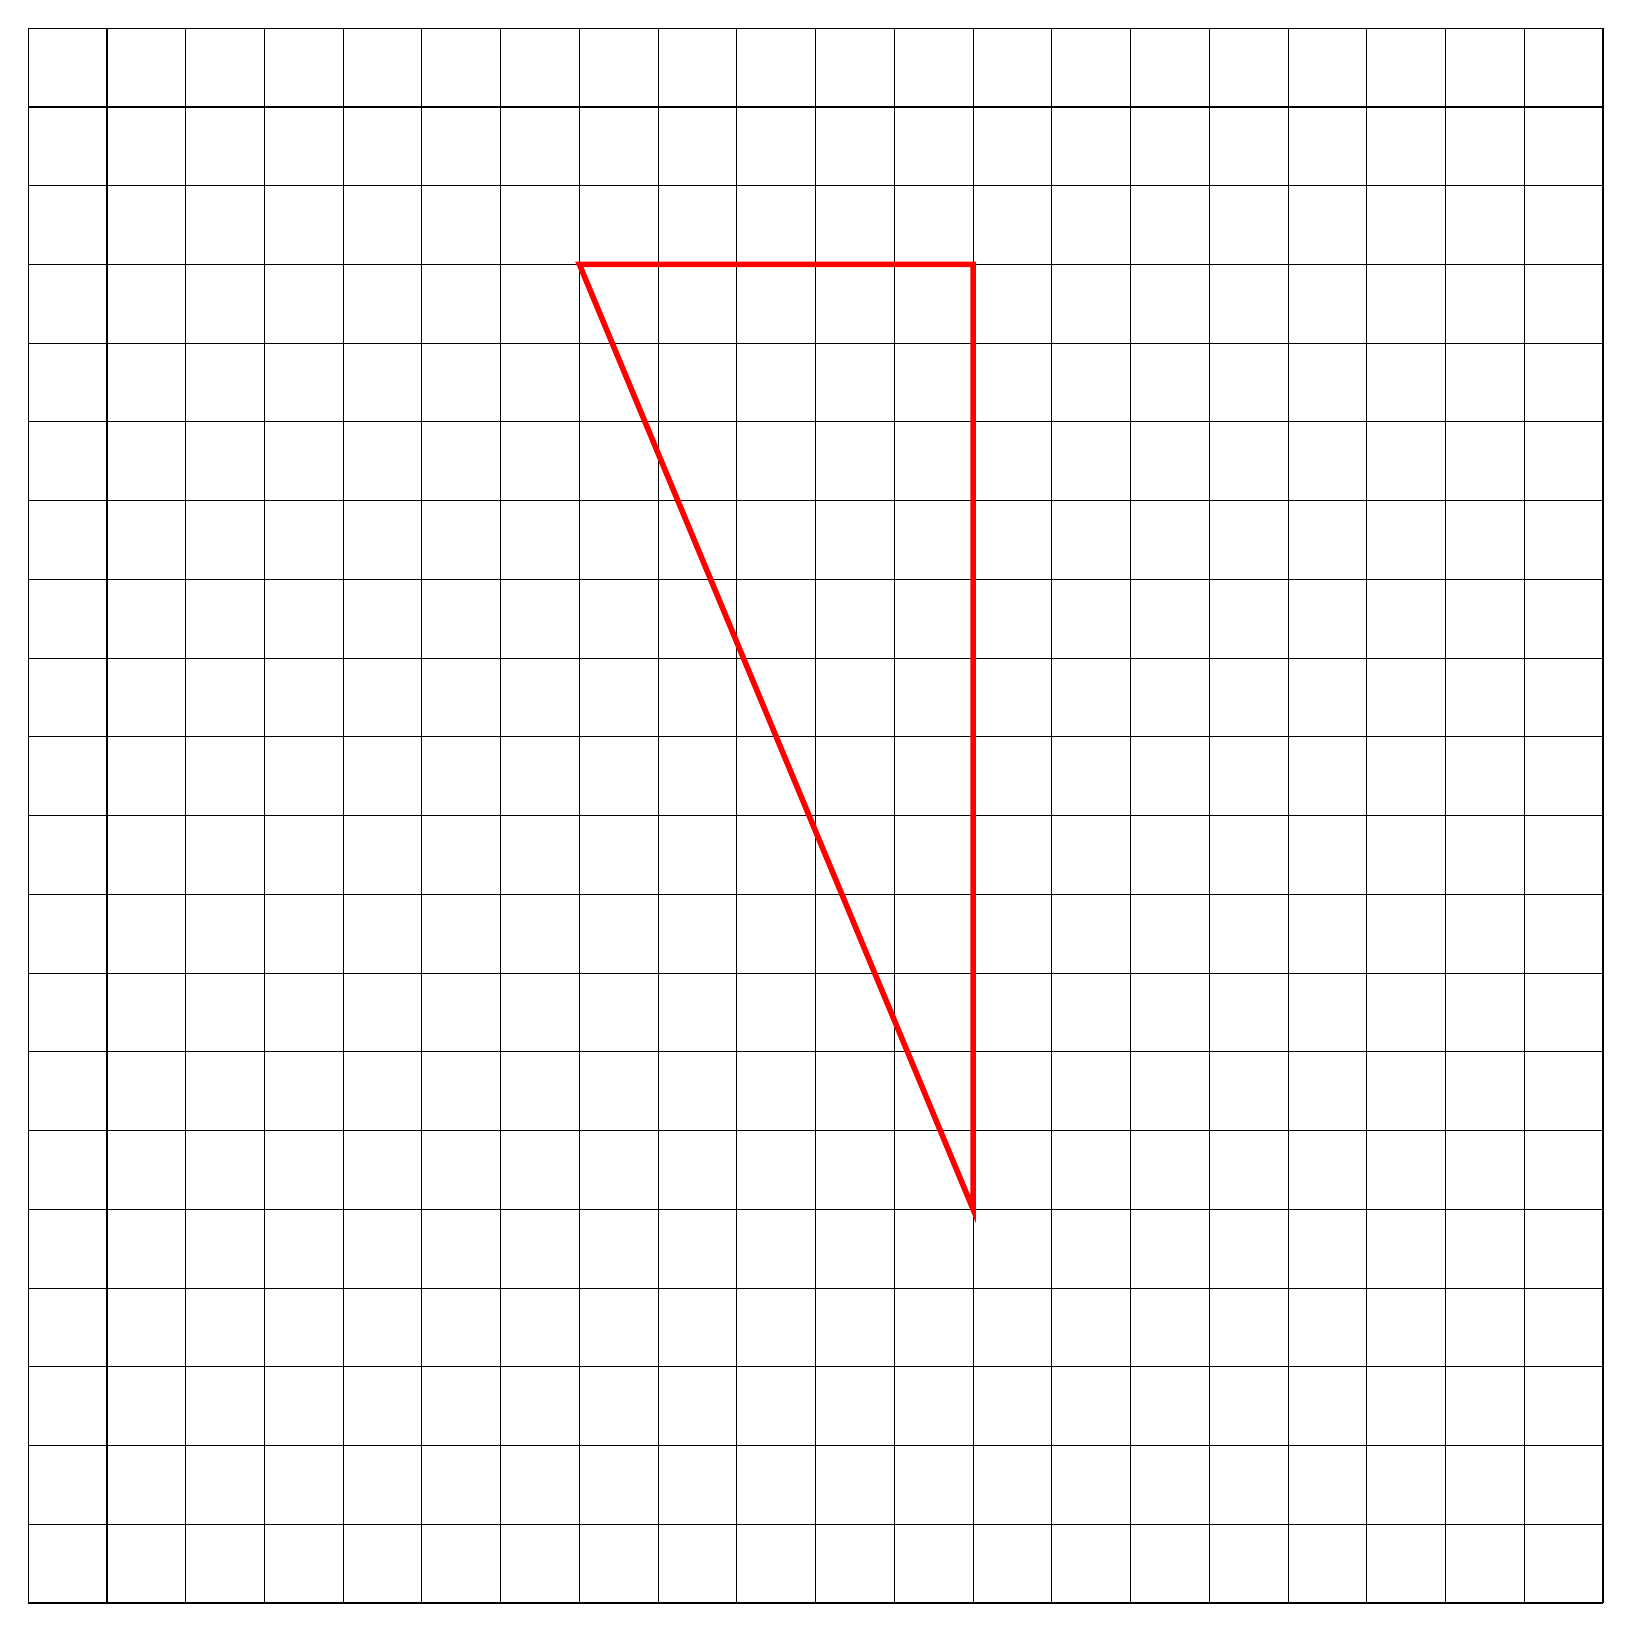
\begin{tikzpicture}
\draw (-10, -10) grid (10, 10);

\coordinate (a) at (2, -5);
\coordinate (b) at (2, 7);
\coordinate (c) at (-3, 7);

\draw [line width=2pt, red] (a) -- (b) -- (c) -- cycle;
\end{tikzpicture}

\[
height = 12, base = 5, hypotenuse = \sqrt{5^2 + 12^2} = \sqrt{25+ 144} = \sqrt{169} = 13
\]

\subsubsection{11}

Find the area of the rectangle whoose vertices are

a) $(4, 1), (-2, 3), (-2, 1), (4, 3) $

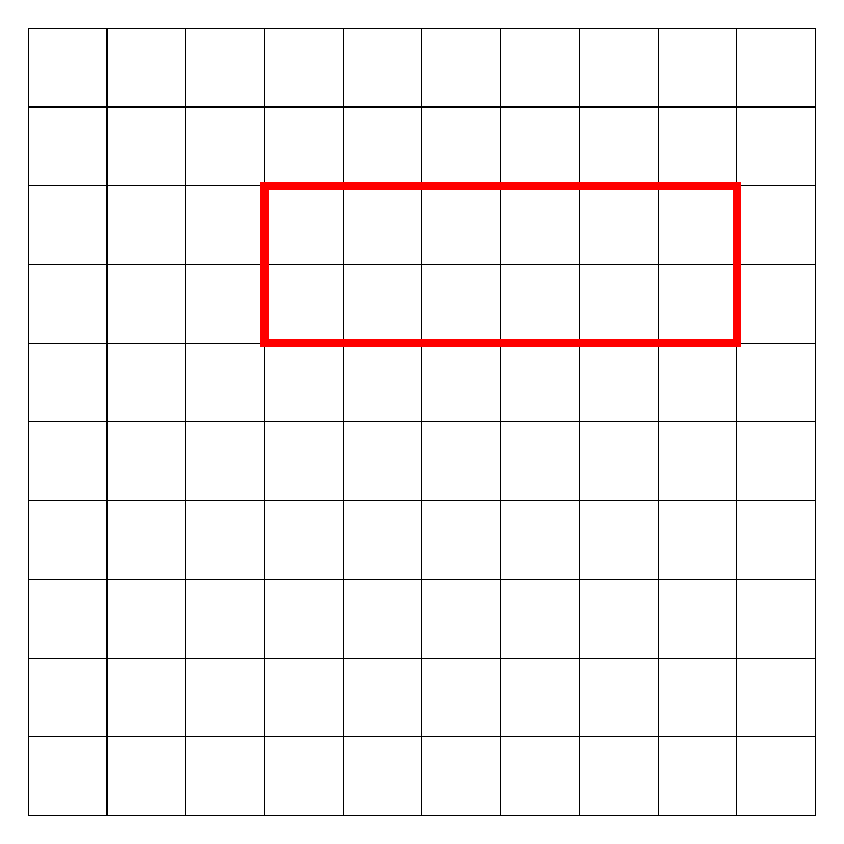
\begin{tikzpicture}
\draw (-5, -5) grid (5, 5);
\coordinate (a) at (4, 1);
\coordinate (b) at (-2, 3);
\coordinate (c) at (-2, 1);
\coordinate (d) at (4, 3);

\draw[line width=3pt, red] (a) -- (d) -- (b) -- (c) -- cycle;


\end{tikzpicture}

\[
height =  3 - 1 = 2, width = 4 - (-2) = 6, area = 2 \cdot 6 = 12
\]


b) $(-3, 7), (4, 2), (-3, 2), (4, 7) $

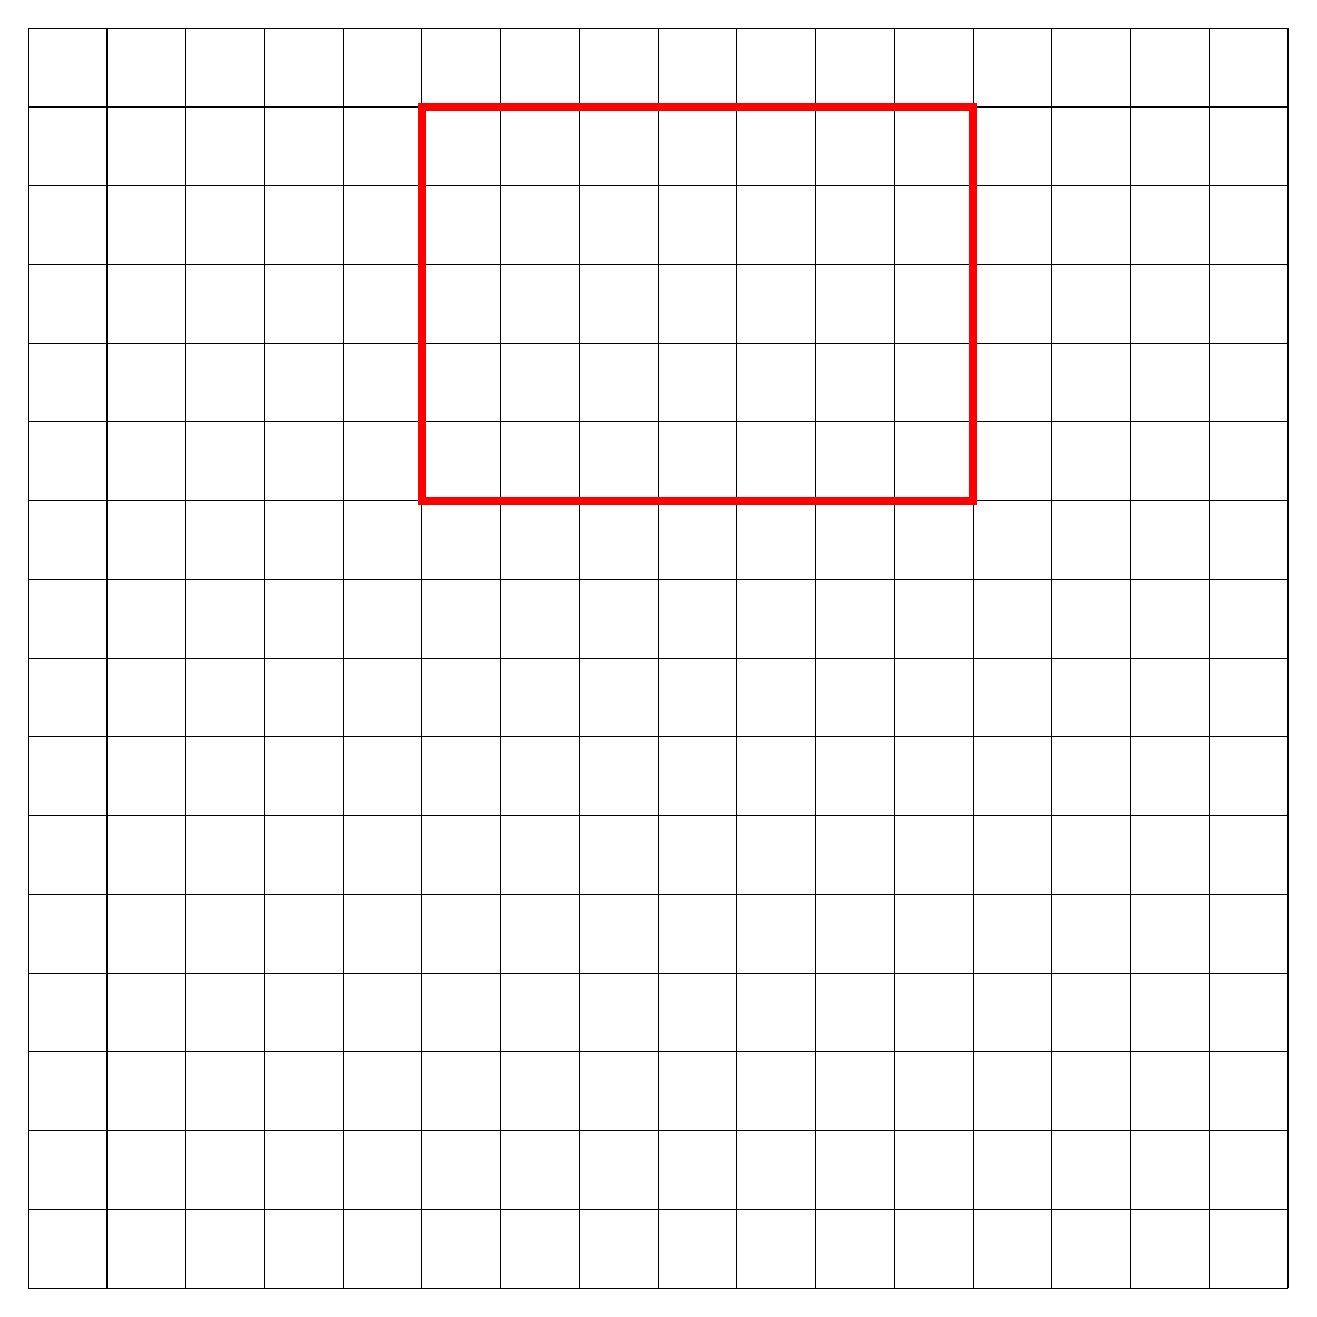
\begin{tikzpicture}
\draw (-8, -8) grid (8, 8);

\coordinate (a) at (-3, 7);
\coordinate (b) at (4, 2);
\coordinate (c) at (-3, 2);
\coordinate (d) at (4, 7);

\draw[line width=3pt, red] (a) -- (d) -- (b) -- (c) -- cycle;

\end{tikzpicture}

\[
height = 7 - 2 =  5, width  = 4 - (-3) = 7, area = 5 \cdot 7 = 35
\]


\subsubsection{12}
Find the coordinates of the midpoint of the segment joining

a) $(0, 0) to (6, 8)$

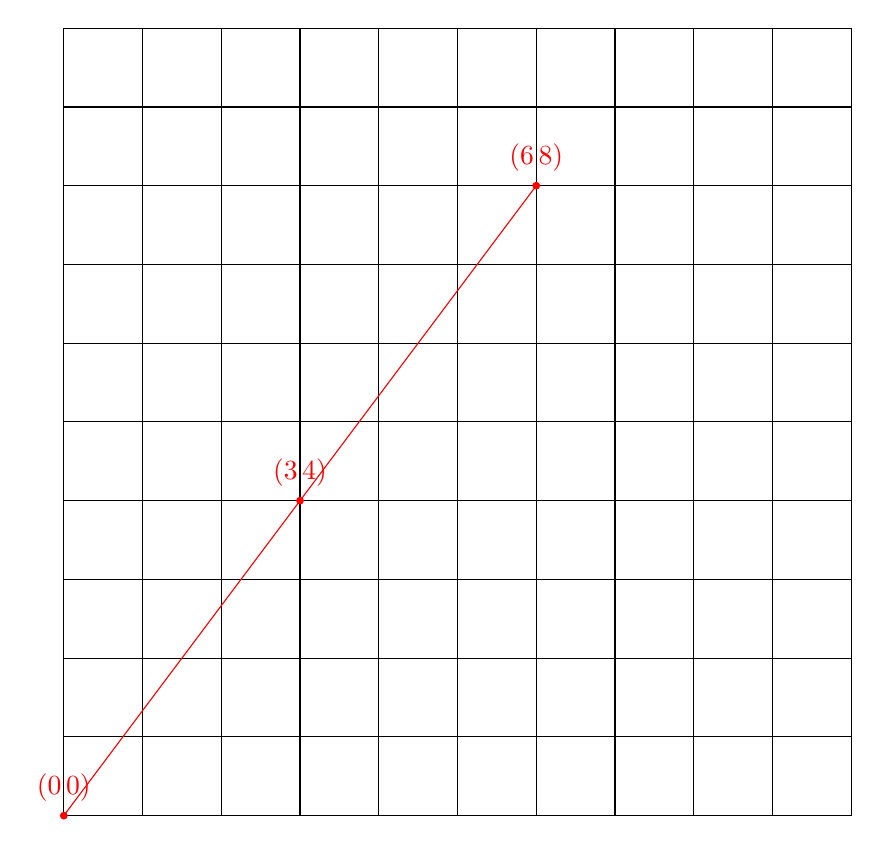
\begin{tikzpicture}
\draw (0, 0) grid (10,10);

\draw[red] (0, 0)  node[circle, fill, inner sep=1pt, label=above:(0\,0)](a){} -- (6, 8) node[circle, fill, inner sep=1pt, label=above:(6\,8)](b){};

\draw[red] (3, 4)  node[circle, fill, inner sep=1pt, label=above:(3\,4)](mid){};

\end{tikzpicture}



\[
midpoint = (0 + \frac{6-0}{2}, 0 + \frac{8-0}{2}) = (3, 4)
\]

b) $(1, 2) to (7, 8)$

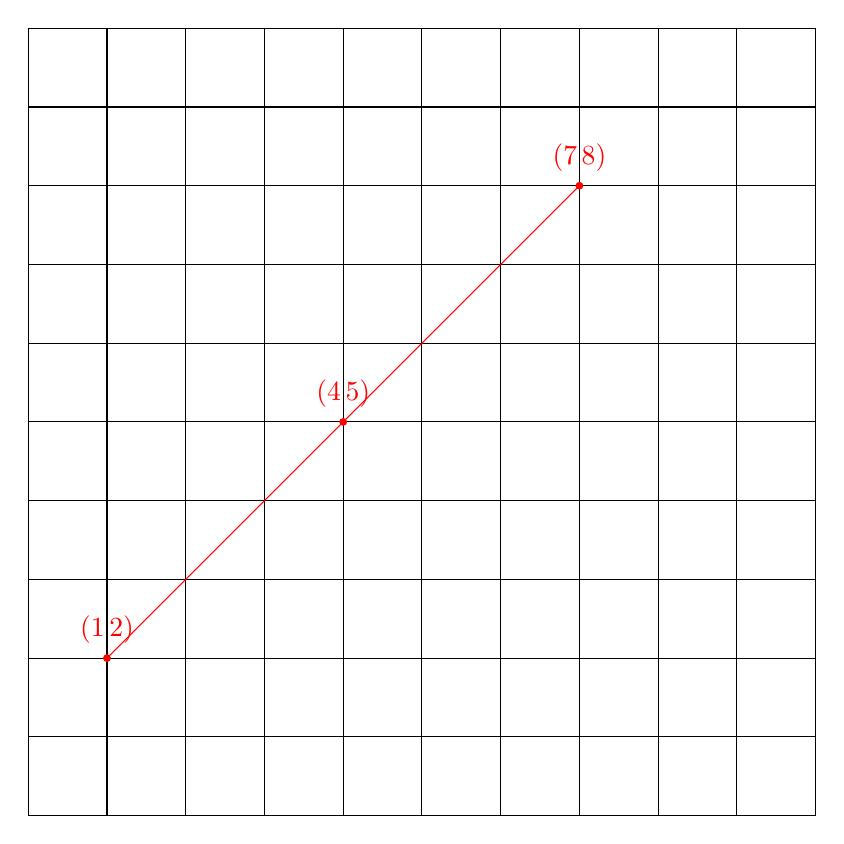
\begin{tikzpicture}
\draw (0, 0) grid (10, 10);

\draw[red] (1, 2) node[circle, fill, inner sep=1pt, label=above:(1\,2)](a){} -- (7, 8) node[circle, fill, inner sep=1pt, label=above:(7\,8)](b){};

\draw[red] (4, 5)  node[circle, fill, inner sep=1pt, label=above:(4\,5)](mid){};
\end{tikzpicture}

\[
midpoint = (1 + \frac{7 - 1}{2}, 2 + \frac{8 - 2}{2}) = (4, 5)
\]

\subsubsection{13}

Sketch on a suitable diagram all points (x, y)
such that

a) $x = 3$


\begin{tikzpicture}
\draw (0, 0) grid (5, 5);

\draw [red] (3, 0) -- (3, 5);

\end{tikzpicture}

b) $y= -4$


\begin{tikzpicture}
\draw (-5, -5) grid (5, 5);

\draw [red] (-5, -4) -- (5, -4);
\end{tikzpicture}

c) $x<3 and y > 2$

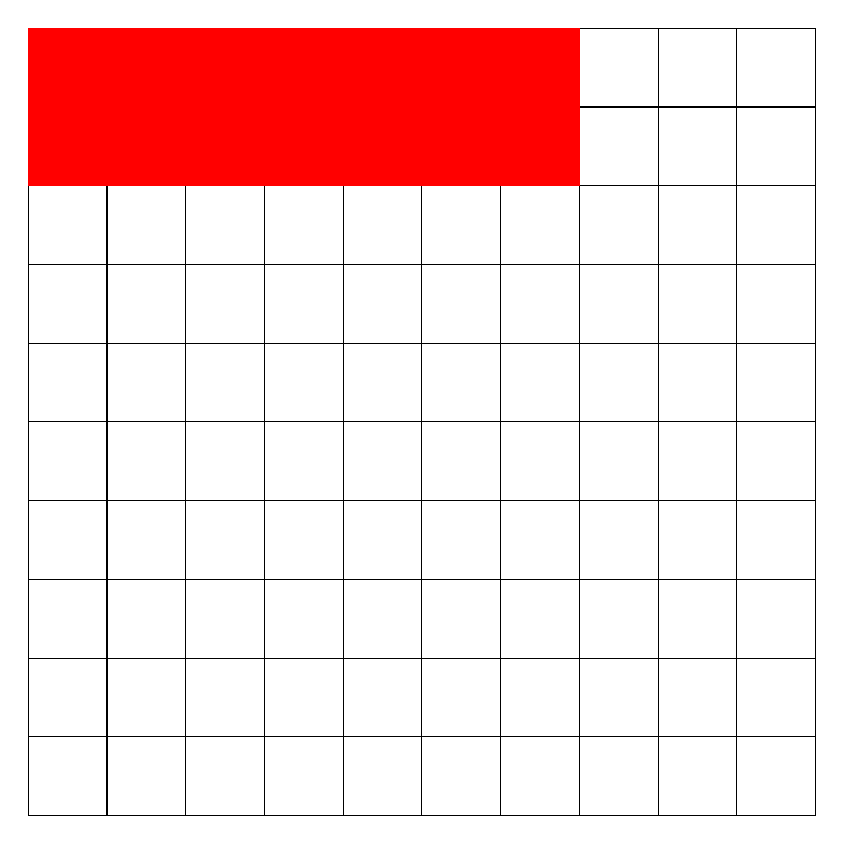
\begin{tikzpicture}
\draw (-5, -5) grid (5, 5);

\draw [red, fill] (-5, 3) -- (2, 3) -- (2, 5) -- (-5, 5) -- cycle;
\end{tikzpicture}

d) x or y (or both) is zero


\begin{tikzpicture}
\draw (-5, -5) grid (5, 5);

\draw [red] (0, 0) -- (5, 0);

\draw [red] (0, 0) -- (0, 5);

\end{tikzpicture}

e) $x >= 0 $ and $y <= 0$

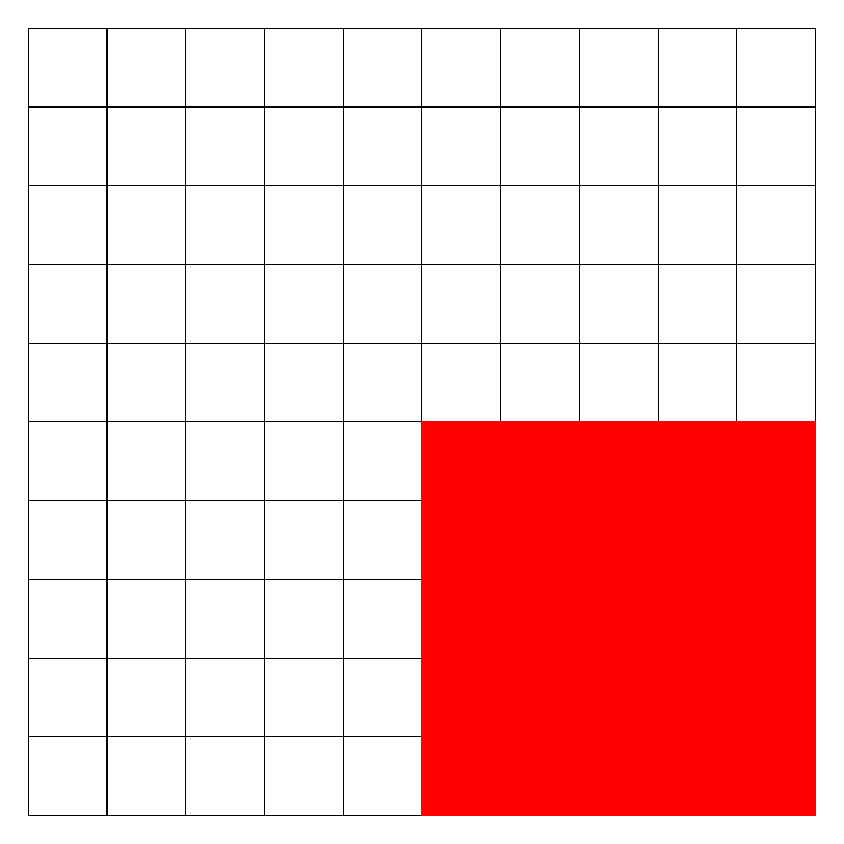
\begin{tikzpicture}
\draw(-5, -5) grid (5, 5);

\draw [red, fill] (0, 0) -- (0, -5) -- (5, -5) -- (5, 0) -- cycle;
\end{tikzpicture}


f) $x^2 <= 1$

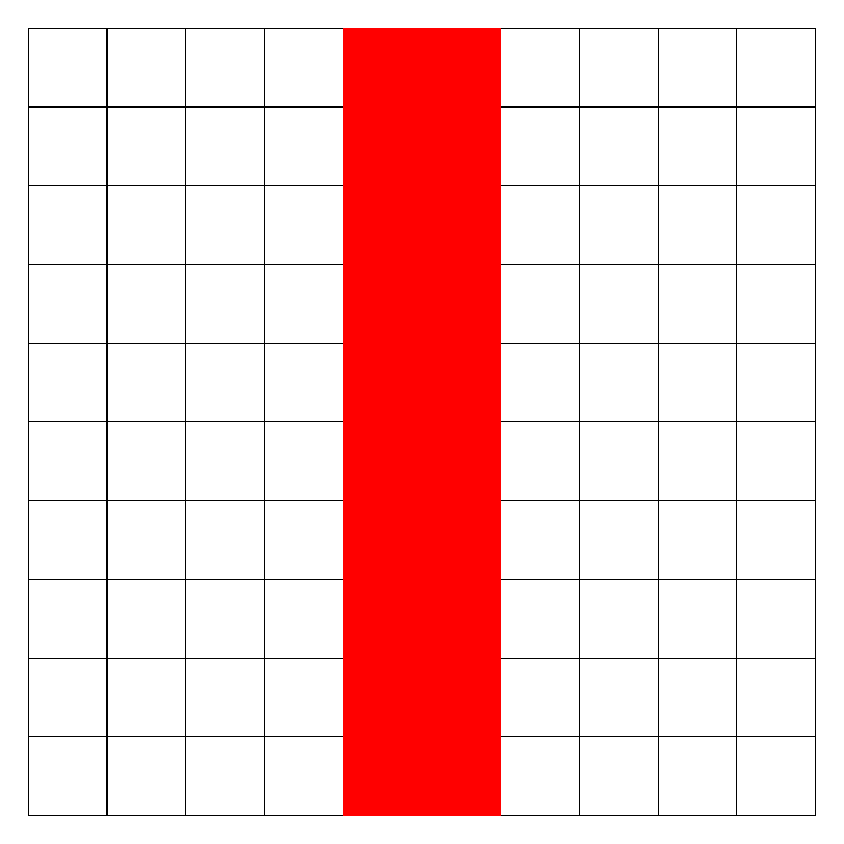
\begin{tikzpicture}
	\draw (-5, -5) grid (5, 5);
	
	\draw [red, fill] (-1, -5) -- (1, -5) -- (1, 5) -- (-1, 5) -- cycle;
\end{tikzpicture}


\subsubsection{14}

Find the slope determined by 

a) $(1, 2)$ and $(3, 6)$

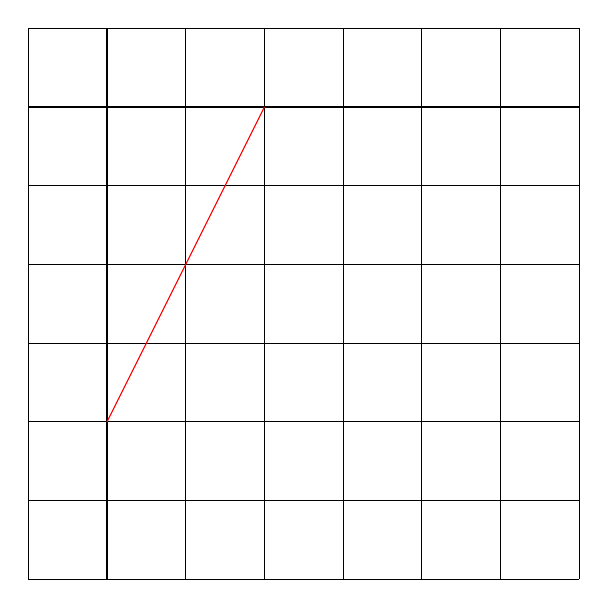
\begin{tikzpicture}
\draw(0, 0) grid (7, 7);

\draw [red](1, 2) -- (3, 6);
\end{tikzpicture}

\[
	m = \frac{6 - 2}{3 - 1} = \frac{4}{2} = 2
\]

b) $(-2, 4)$ and $(3, 4)$


\begin{tikzpicture}
\draw (-5,-5 ) grid (5, 5);

\draw [red] (-2, 4) -- (3, 4);
\end{tikzpicture}

\[
m = \frac{3 - (-2)}{4-4} = 0
\]

c) $(-2, 1)$ and $(2, -3)$

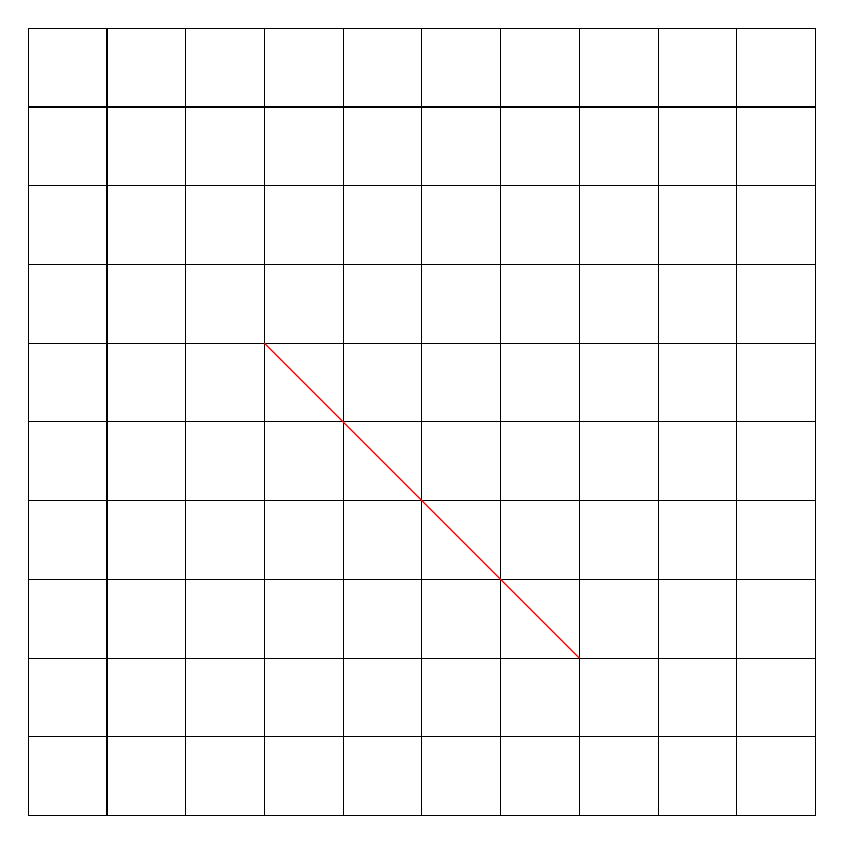
\begin{tikzpicture}
\draw(-5, -5) grid (5, 5);

\draw [red] (-2, 1) -- (2, -3);
\end{tikzpicture}

\[
	m = \frac{-3 - 1}{2 - (-2)} = \frac{-4}{4} = -1 
\]


\subsubsection{15}

Find the equation of the line through

a) $(-1, -2)$ and $(1, 0)$

\[
m = \frac{0 - (-2)}{1 - (-1)} = \frac{2}{2} = 1; 0 = 1 \cdot 1 + c; c = -1; y = x - 1
\]

b) $(0, 4)$ and $(1, 7)$

\[
m = \frac{7 - 4}{1 - 0} = \frac{3}{1} = 3; c = 7 - 3\cdot 1 = 4; y = 3x + 4
\]

c) $(4, -2)$ and $(4, 19)$

\[
m = \frac{19 - (-2)}{4 - 4} = 0; x = 4
\]


\subsubsection{16}

Show that the lines $3x + y = 2$ and $2y = 1- 6x$ are parallel

\begin{align*}
3x + y = 2 \tag{Equation 1}\\
y = -3x + 2 \tag{when rearranged}\\
\\
2y = 1 - 6x \tag{Equation 2}	\\
y = \frac{1 - 6x}{2} = \frac{1}{2} - 3x \tag{when rearranged}
\end{align*}

Given Equation 1 and Equation 2 have same slope, they will never intercept unless they are the same line, but given the y intercepts are different, then they aren't the same line. Meaning the cross the y axis at different points and slope in same direction


\subsubsection{17}

Write the equation of the line through (-2, -3) which is 

a) parallel to $x + 2y = 3$

Rearranging, we get $y = \frac{3 - x}{2}$

For the line to be parallel, the slope will be the same, thus $m=\frac{1}{2}$ The y intercept $c$ will be $-3 = \frac{1}{2}\cdot -2 + c; c=-2$

\[
	y = \frac{1}{2}x -2
\]

b) perpendicular to $x + 2y = 3$

Rearranging, we get $y = \frac{3 - x}{2}$

For the line to be perpendicular, the slope will now be different. Lets call the slope of the original equation, $m_1$ and the slope of the perpendicular equation, $m_2$. And that two slopes being perpendicular satisfy $m_1\cdot m_2 = -1$

Thus the slope of the perpendicular line, is $-\frac{1}{2}m_2 = -1$ or $m_2 = 2$

now for the point $(-2, -3)$ we have $ -3 = 2 \cdot (-2) + c$ or $c = 1$

So the perpendicular line is

$y = 2x + 1$


\subsubsection{18}

Write the equation of the circle with

a) center (0,0) and radius 2;

$ (x + 0)^2 + (y+0)^2 = x^2 + y^2 = 2^2$


b) center (-2,0) and radius 7;

$(x+2)^2 +y^2 = 49$

c) center (3,6) and radius $\frac{1}{2}$;

$(x-3)^2 + (y-6)^2 = \frac{1}{4}$

d) with (5, 5) and (-3, -1) as the ends of a diameter

Proposing we draw a straight line from $(5, 5)$ to $(-3, -1)$, the midpoint indicates the center.
$(\frac{5-3}{2}, \frac{5-1}{2}) = (1, 2)$

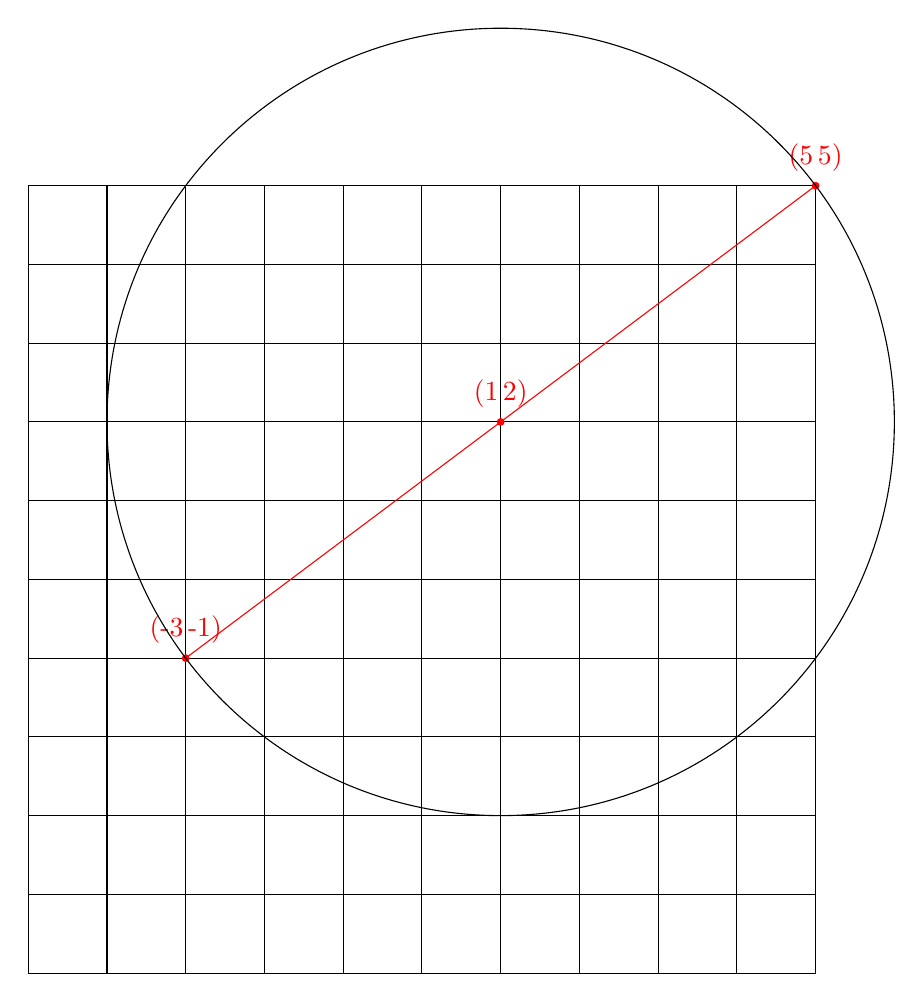
\begin{tikzpicture}
\draw (-5, -5) grid (5, 5);


\draw[red] (-3, -1)  node[circle, fill, inner sep=1pt, label=above:(-3\,-1)](a){} -- (5, 5) node[circle, fill, inner sep=1pt, label=above:(5\,5)](b){};

\draw[red] (1, 2)  node[circle, fill, inner sep=1pt, label=above:(1\,2)](mid){};

\draw (1, 2) circle (5);

\end{tikzpicture}

thus the equation of the ciircle is 

\[
(x-1)^2 + (y-2)^2 = 25
\]

\subsubsection{19}

Find the center and radius of the circle whose equation is

a) $(x + 3)^2 + (y - 6) ^2 = 9$

$r = \sqrt{9} = 3$

$center = (-3, +6)$


b) $(x - 4)^2 + (y) ^2 = 4$

$r = 2$

$center = (4, 0)$


c) $(x )^2 + (y + 2) ^2 = 1$

$r = 1$

$center = (0, -2)$


d) $x^2 + y^2 + 6x + 2y + 6  = 0$
\begin{align*}
	x^2 + y^2 + 6x + 2y + 6  = 0 \tag{1} \\
	(x + 3)^2 + (y+1)^2  -4 = 0  \tag{factoring out x and y} \\
	(x + 3)^2 + (y+1)^2 = 4
\end{align*}

Thus, $radius = \sqrt{4} = 2$ and $center = (-3, -1)$

e) $x^2 + y^2 - 16x + 14y + 97 = 0$

\begin{align*}
x^2 + y^2 - 16x + 14y + 97 = 0	\tag{1} \\
x^2 - 16x + 48 + (y + 7)^2 = 0 \tag{factoring out y}\\
(x-8)^2 + (y+7)^2 - 16 = 0 \tag{factoring out x} \\
(x-8)^2 + (y+7)^2 = 16
\end{align*}

Thus $radius = \sqrt{16} = 4$ and center $(8, -7)$

\subsubsection{20}

On a single set of coordinate axes, sketch the line $x + 16 = 7y$ and the circle $x^2 + y^2 - 4x + 2y = 20$ and find their points of intersection.

\begin{align*}
	x + 16 = 7y \tag{1} \\
	x = 7y - 16 \tag{rearranging} \\
	x^2 + y^2 - 4x + 2y = 20  \tag{2} \\
	(7y - 16)^2 + y^2 - 4(7y -16) + 2y = 20 \tag{eliminating x} \\
	49y^2 - 224y + 256 + y^2 - 28y  + 64 + 2y = 20 \tag{expanding} \\
	50y^2 - 250y + 320 = 20 \\
	50y^2 - 250y + 300 = 0 \\
	y = \frac{250 \pm \sqrt{(-250)^2 - 4 \cdot 50 \cdot 300}}{2 \cdot 50} \\
	y = \frac{250 \pm \sqrt{2500}}{100} = \frac{250 \pm 50}{100}\\
	y = \frac{200}{100} = 2, or, y = \frac{300}{100} = 3
\end{align*}

Thus, when $y = 2$, $x = 7\cdot 2 - 16 = -2$ and when $y = 3$ then $x = 7\cdot 3 -16 = 5$

So the points on intersection are, (-2, 2) and (5, 3)


\subsubsection{21}
Find the focus and directrix of each of the following parabolas

a) $ y = 2x^2$

b) $y = \frac{1}{8}x^2$

c) $y = -5x^2$

d) $y = -\frac{1}{12}x^2$

\subsubsection{22}

A parabola has vetical axis and vertex at the origin.

Write its equation if its focus is at 

a) $(0, 3)$

b) $(0, 16)$

c) $(0, -1)$

d) $(0, -\frac{1}{10})$

\subsubsection{23}

Find the vertex and focus of each of the following parabolas, and state whether it opens up or down;

a) $y = x^2 - 4x + 1$

b) $y = 2x^2 - 12x - 7 $

c) $y = -x^2 -4x + 5$

d) $y = 4 - 2x - \frac{1}{2} x^2$

\end{document}

